\section{Obtención de características}
\begin{frame}
 \tableofcontents[currentsection,hideothersubsections]    
\end{frame}

\begin{frame}{Obtención de características}
 \begin{columns}[t]
  \column{.5\textwidth}
  \begin{block}{Categorías}
   	\begin{itemize}
	\item acuático
	\item nieve
	\item equipo
	\item raqueta
	\item precisión
	\item motor
	\item atletismo
	\item combate
	\end{itemize}
  \end{block}
  \column{.5\textwidth}
  \begin{block}{Instalaciones}
  	\begin{itemize}
	\item campo césped
	\item campo tierra
	\item pista hielo
	\item pista césped
	\item pista tierra
	\item pista dura
	\item cancha parqué
	\item ...
	\end{itemize}
  \end{block}
 \end{columns}
\end{frame}

\begin{frame}{Obtención de características II}
 \begin{columns}[t]
  \column{.5\textwidth}
  \begin{block}{Accesorios}
   	\begin{itemize}
	\item cuerda
	\item pesas
	\item bate
	\item casco
	\item raqueta
	\item pala
	\item balón
	\item pelota
	\end{itemize}
  \end{block}
  \column{.5\textwidth}
  \begin{block}{Otros}
  	\begin{itemize}
	\item caballo
	\item barco
	\item coche
	\item moto
	\item avión
	\item globo
	\end{itemize}
  \end{block}
 \end{columns}
\end{frame}


\begin{frame}{Obtención de características III}
\begin{figure} [ht]
\begin {center}
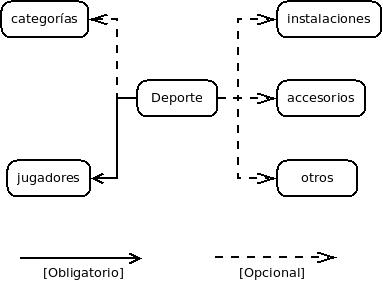
\includegraphics[scale = 0.4]{./../doc/Deportes.jpeg}
\caption{Diagrama de relación entre objetos y propiedades}
\end {center}
\end{figure}
\end{frame}
